\section{Backlog/roadmap du sprint Production}

L’objectif de ce sprint est de finaliser en augmentant encore la valeur donné à l'utilisateur par:
Ajout de deux fonctionnalités concernant les dispositions symétriques. L’objectif étant d'éliminer ces dispositions
symétriques qui apportent peu, voire prêtent à confusion pour l’utilisateur.
Dernière amélioration mineure de l’interface, surtout sur le visuel, pour aligner le design des messages de réponse
à celui de l’interface principale.\\

Pour ce faire le backlog suivant a été \emph{embarqué} dans cette version et a résulté en la roadmap suivante:


\begin{center}
    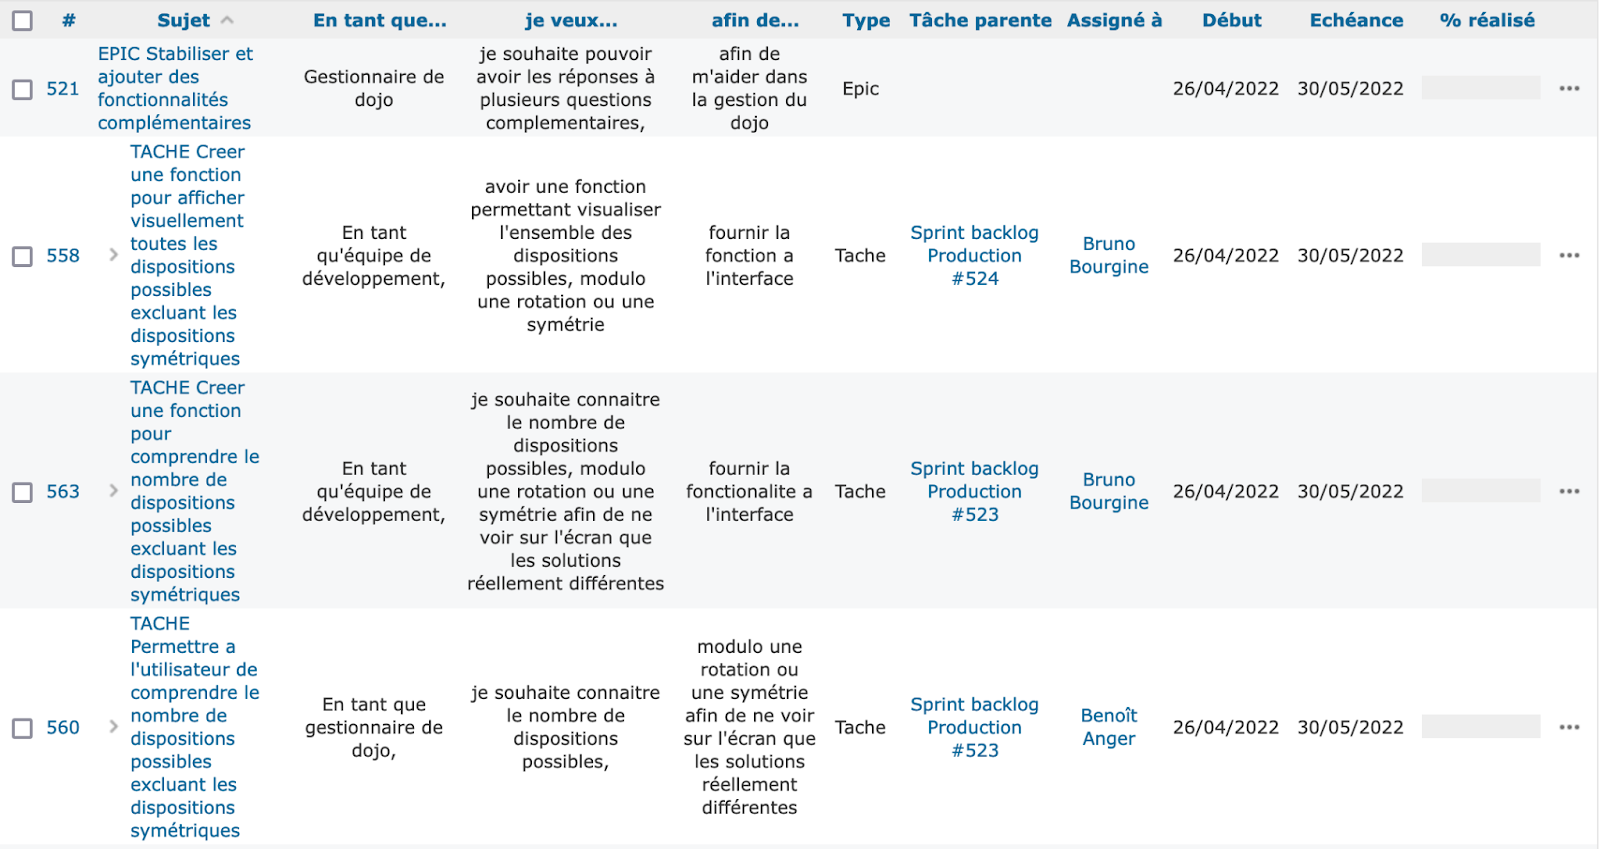
\includegraphics[width=17cm]{images/roadmap-prod-part1.png}
\end{center}

\begin{center}
    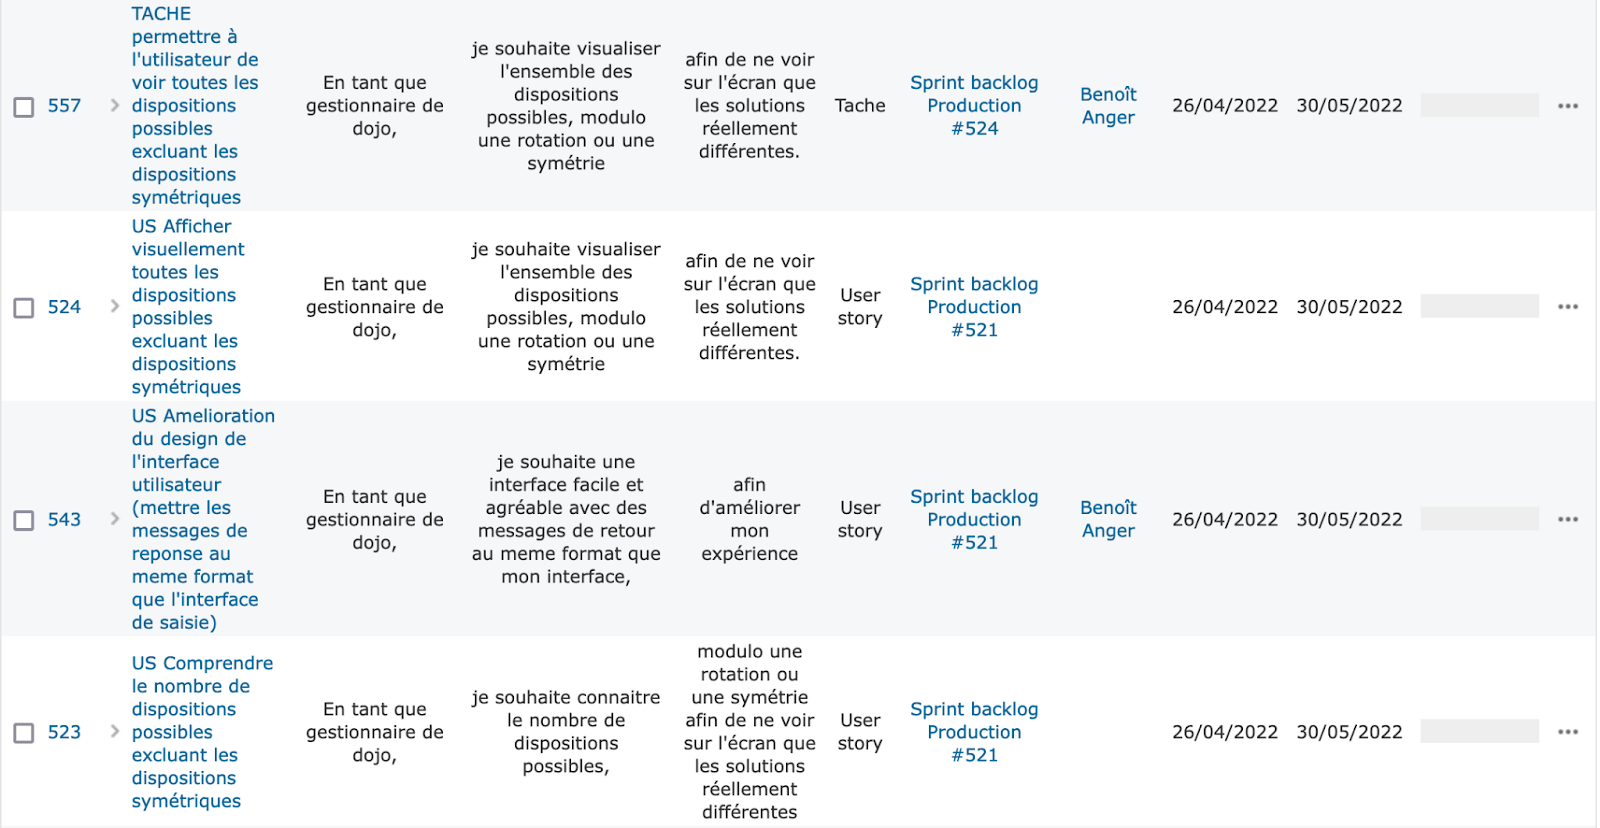
\includegraphics[width=17cm]{images/roadmap-prod-part2.png}
    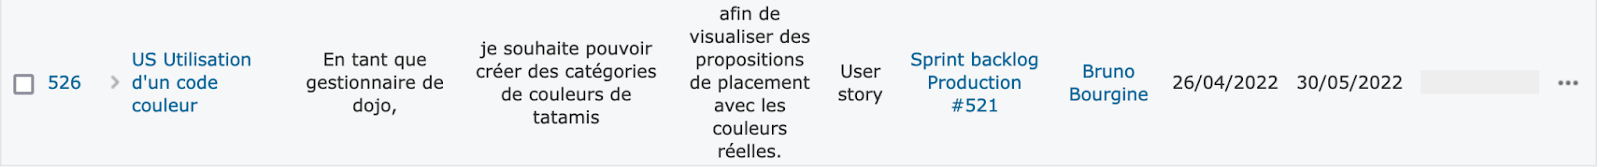
\includegraphics[width=17cm]{images/roadmap-prod-part3.png}
\end{center}

\bigskip

Et ici présenté en diagramme de Gantt:

\begin{center}
    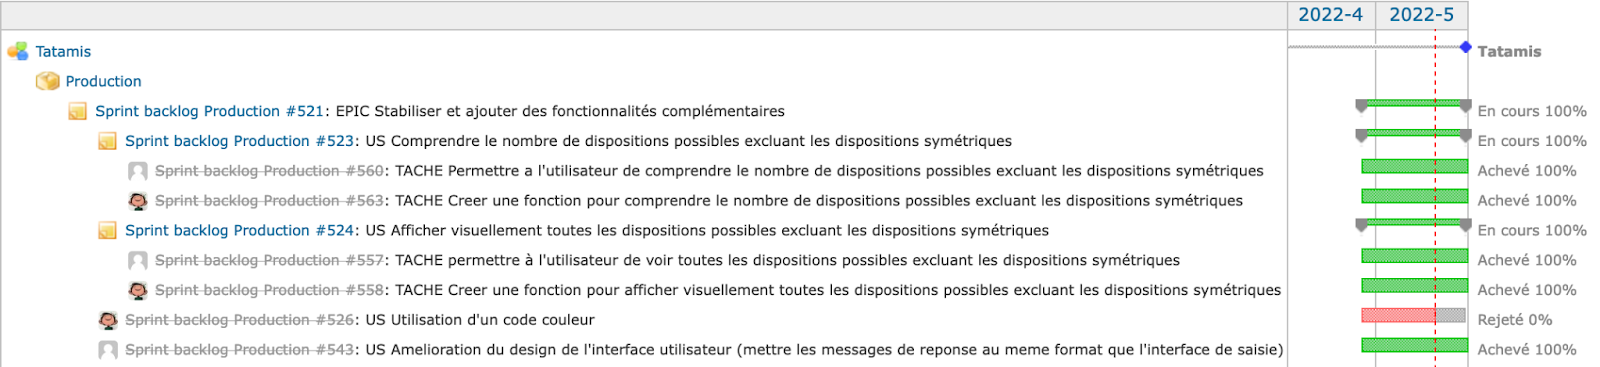
\includegraphics[width=17cm]{images/tatamis-gantt-prod.png}
\end{center}

\section{Tests}

Les tests réalisés pour cette version et leurs résultats sont les suivants:\\


\noindent%
\begin{adjustwidth}{-1.5cm}{0cm}

    \renewcommand{\arraystretch}{1.2}
    {\setlength{\tabcolsep}{1.5 mm}
        \begin{testtabular}{|m{0.6cm}|m{5.5cm}|m{8cm}|m{2cm}|c|} \hline
            \rowcolor{tssteelblue} \textcolor{white}{id}                        & \textcolor{white}{Sujet}                                                                   & \textcolor{white}{Test d'acceptance (en gris : test utilisateur)}                                                                                            & \textcolor{white}{Méthode de test} & \textcolor{white}{Résultat} \\ \hline
            523 & US Comprendre le nombre de dispositions possibles excluant les dispositions symétriques                & Étant donné que l'utilisateur saisie des dimensions valides de dojo, il obtient le nombre de solutions possibles en excluant les solutions symétriques                                                   & Manuel          & OK       \\ \hline
            524 & US Afficher visuellement toutes les dispositions possibles excluant les dispositions symétriques       & \cellcolor{tsgrey} Étant donné des dimensions d'un dojo saisies, quand il sélectionne cette option, il obtient visuellement toutes les dispositions possibles en excluant les solutions symétriques      & Manuel          & OK       \\ \hline
        \end{testtabular}}
\end{adjustwidth}

\bigskip

Par ailleurs, étant donné qu’il s’agit de la dernière version pour mise en production, il est important de tester
l’ensemble des fonctionnalités du programme. Des tests de non régression ont été effectués:\\

\noindent%
\begin{adjustwidth}{-1.5cm}{0cm}

    \renewcommand{\arraystretch}{1.2}
    {\setlength{\tabcolsep}{1.5 mm}
        \begin{testtabular}{|m{5cm}|m{5cm}|m{1.5cm}|m{1.5cm}|m{1.5cm}|m{3cm}|} \hline
            \rowcolor{tssteelblue}  \textcolor{white}{Sujet}    & \textcolor{white}{Test d'acceptance}   & \textcolor{white}{Rédacteur cahier de tests}   & \textcolor{white}{Méthode de test}  & \textcolor{white}{Testeur} & \textcolor{white}{Résultat} \\ \hline
            Champs de saisie \emph{Longueur} - test de saisie $>$ 25 (26)&Saisie impossible&Benoit&Manuel&Benoit&OK avec version 5.9.7 de PyQt \tabularnewline & & & & & KO avec version 5.12.2 de PyQt \\ \hline
            Champs de saisie \emph{Largeur} - test de saisie $>$  25 (26)&Saisie impossible&Benoit&Manuel&Benoit&OK avec version 5.9.7 de PyQt \tabularnewline & & & & & KO avec version 5.12.2 de PyQt\\ \hline
            Champs de saisie \emph{Nombre de tatamis disponibles} - test de saisie $>$ 300 (301)&Saisie impossible&Benoit&Manuel&Benoit&OK avec version 5.9.7 de PyQt \tabularnewline & & & & & KO avec version 5.12.2 de PyQt\\ \hline
            Champs de saisie \emph{Longueur} - test de saisie nulle (puis cliquer sur chaque boutons - sauf le dernier bouton du bas liee a une autre saisie)&Message d'erreur "Erreur de saisie des dimensions Aucune dimension ne peut avoir une valeur nulle ou vide"&Benoit&Manuel&Bruno&OK\\ \hline
            Champs de saisie \emph{Longueur} - test d'absence de saisie (puis cliquer sur chaque boutons - sauf le dernier bouton du bas liee a une autre saisie)&Message d'erreur "Erreur de saisie des dimensions Aucune dimension ne peut avoir une valeur nulle ou vide"&Benoit&Manuel&Bruno&OK\\ \hline
            Champs de saisie \emph{Largeur} - test de saisie nulle (puis cliquer sur chaque boutons - sauf le dernier bouton du bas liee a une autre saisie)&Message d'erreur "Erreur de saisie des dimensions Aucune dimension ne peut avoir une valeur nulle ou vide"&Benoit&Manuel&Bruno&OK\\ \hline
            Champs de saisie \emph{Largeur} - test d'absence de saisie (puis cliquer sur chaque boutons - sauf le dernier bouton du bas liee a une autre saisie)&Message d'erreur "Erreur de saisie des dimensions Aucune dimension ne peut avoir une valeur nulle ou vide"&Benoit&Manuel&Bruno&OK\\ \hline
            Champs de saisie \emph{Nombre de tatamis disponibles} - test de saisie nulle puis cliquer sur le bouton "Obtenir une solution etant donne un nombre de tatamis"&Message d'erreur "Erreur de saisie des dimensions Aucune dimension ne peut avoir une valeur nulle ou vide"&Benoit&Manuel&Bruno&OK\\ \hline
            Champs de saisie \emph{Nombre de tatamis disponibles} - test d'absence de saisie puis cliquer sur le bouton "Obtenir une solution etant donne un nombre de tatamis"&Message d'erreur "Erreur de saisie des dimensions Aucune dimension ne peut avoir une valeur nulle ou vide"&Benoit&Manuel&Bruno&OK\\ \hline
            Fonctionnalité "Afficher la surface du dojo" en saisissant des dimensions valides (3,1)&Réponse: La surface du dojo est 3.&Benoit&Manuel&Benoit&OK\\ \hline
        \end{testtabular}}
\end{adjustwidth}

\noindent%
\begin{adjustwidth}{-1.5cm}{0cm}

    \renewcommand{\arraystretch}{1.2}
    {\setlength{\tabcolsep}{1.5 mm}
        \begin{testtabular}{|m{5cm}|m{5cm}|m{1.5cm}|m{1.5cm}|m{1.5cm}|m{3cm}|} \hline
            \rowcolor{tssteelblue}  \textcolor{white}{Sujet}    & \textcolor{white}{Test d'acceptance}   & \textcolor{white}{Rédacteur cahier de tests}   & \textcolor{white}{Méthode de test}  & \textcolor{white}{Testeur} & \textcolor{white}{Résultat} \\ \hline
            Fonctionnalité "Savoir si il existe une disposition pour ce dojo" en saisissant des dimensions ou il existe (3,4)&Réponse: Il existe au moins une disposition avec des tatamis 2 $\times$ 1 pour ce dojo&Benoit&Manuel&Benoit&OK\\ \hline
            Fonctionnalité "Savoir si il existe une disposition pour ce dojo" en saisissant des dimensions ou il n'existe pas (3,1)&Réponse: Il n'existe pas de disposition possible avec des tatamis 2 $\times$ 1 pour ce dojo&Benoit&Manuel&Benoit&OK\\ \hline
            Fonctionnalité "Connaître le nombre de dispositions possibles" en saisissant des dimensions ou il n'existe pas de disposition (3,1)&Réponse: Il existe 0 disposition possible&Benoit&Manuel&Benoit&OK\\ \hline
            Fonctionnalité "Connaître le nombre de dispositions possibles" en saisissant des dimensions ou il existe au moins une disposition (3,4)&Réponse: Il existe 4 dispositions possibles&Benoit&Manuel&Benoit&OK\\ \hline
            Fonctionnalité "Connaître le nombre de tatamis 2 $\times$ 1 nécessaires pour la taille du dojo" en saisissant des dimensions ou il existe au moins une disposition (3,4)&Réponse: Le nombre de tatamis 2 $\times$ 1 nécessaires pour ce dojo est : 6&Benoit&Manuel&Benoit&OK\\ \hline
            Fonctionnalité "Connaître le nombre de tatamis 2 $\times$ 1 nécessaires pour la taille du dojo" en saisissant des dimensions ou il n'existe pas de disposition (3,1)&Réponse: Demande impossible Il n'existe pas de disposition possible avec des tatamis 2 $\times$ 1 pour ce dojo&Benoit&Manuel&Benoit&OK\\ \hline
            Fonctionnalité "Quelle taille maximum de dojo pour avoir une solution?" en saisissant des dimensions ou il n'existe pas de disposition (3,1)&Réponse: La taille maximale est (1, 2)&Benoit&Manuel&Benoit&OK\\ \hline
            Fonctionnalité "Quelle taille maximum de dojo pour avoir une solution?" en saisissant des dimensions ou il existe au moins une disposition (3,4)&Réponse: Demande impossible Il existe au moins une disposition possible avec des tatamis 2 $\times$ 1 pour ce dojo&Benoit&Manuel&Benoit&OK\\ \hline
            Fonctionnalité "Existe-t-il une solutions avec des demi-tatamis?" en saisissant des dimensions ou il n'existe pas de disposition (3,1)&Réponse: Oui&Benoit&Manuel&Benoit&OK\\ \hline
            Fonctionnalité "Existe-t-il une solutions avec des demi-tatamis?" en saisissant des dimensions ou il existe au moins une disposition (3,4)&Réponse: Demande impossible Il existe au moins une disposition possible avec des tatamis 2 $\times$ 1 pour ce dojo&Benoit&Manuel&Benoit&OK\\ \hline
            Fonctionnalité "Afficher une disposition" en saisissant des dimensions ou il existe au moins une disposition (3,4)&Réponse: Affichage d'une disposition avec les indications "Dojo de dimension : 4 x 3 $|$ Surface: 12 $m^2$ $|$ 6 tatamis"&Benoit&Manuel&Benoit&OK\\ \hline
            Fonctionnalité "Afficher une disposition" en saisissant des dimensions ou il n'existe pas de disposition (3,1)&Réponse: Demande impossible Il n'existe pas de disposition possible avec des tatamis 2 $\times$ 1 pour ce dojo&Benoit&Manuel&Benoit&OK\\ \hline

        \end{testtabular}}
\end{adjustwidth}

\noindent%
\begin{adjustwidth}{-1.5cm}{0cm}

    \renewcommand{\arraystretch}{1.2}
    {\setlength{\tabcolsep}{1.5 mm}
        \begin{testtabular}{|m{5cm}|m{5cm}|m{1.5cm}|m{1.5cm}|m{1.5cm}|m{3cm}|} \hline
            \rowcolor{tssteelblue}  \textcolor{white}{Sujet}    & \textcolor{white}{Test d'acceptance}   & \textcolor{white}{Rédacteur cahier de tests}   & \textcolor{white}{Méthode de test}  & \textcolor{white}{Testeur} & \textcolor{white}{Résultat} \\ \hline
            Fonctionnalité "Afficher toutes les dispositions possibles" en saisissant des dimensions ou il existe au moins une disposition (3,4)&Réponse: Affichage de 4 dispositions avec les indications "Dojo de dimension : 4 x 3 $|$ Surface: 12 $m^2$ $|$ 6 tatamis"&Benoit&Manuel&Benoit&OK\\ \hline
            Fonctionnalité "Afficher toutes les dispositions possibles" en saisissant des dimensions ou il n'existe pas de disposition (3,1)&Réponse: Demande impossible Il n'existe pas de disposition possible avec des tatamis 2 $\times$ 1 pour ce dojo&Benoit&Manuel&Benoit&OK\\ \hline
            Fonctionnalité "Obtenir une solution étant donne un nombre de tatamis" en saisissant une dimension valide (23)&Réponse: Dimension(s) possible(s) du dojo étant donné le nombre de tatamis saisi. Ces propositions satisfont aux conditions suivantes:
            \begin{itemize}
                \item un ratio maximum de 3 entre la longueur et la largeur
                \item une utilisation de minimum 75\% des tatamis saisis
            \end{itemize}
            8 $\times$ 5 ; 11 $\times$ 4 ; 7 $\times$ 6 ; 10 $\times$ 4 ; 9 $\times$ 4 ; 6 $\times$ 6
            &Benoit&Manuel&Benoit&OK \\ \hline
            Fonctionnalité "Obtenir une solution étant donne un nombre de tatamis" en saisissant une dimension non valide (2)&Réponse: Demande impossible Saisir au minimum 3 tatamis pour utiliser cette fonctionnalité.&Benoit&Manuel&Benoit&OK\\ \hline

        \end{testtabular}}
\end{adjustwidth}

\bigskip
Erreur sur validation des saisies:

Une erreur a été constaté suivant les versions utilisés de PyQt:
\begin{itemize}
    \item Version 5.9.7: la validation de la saisie des données fonctionne (comportement attendu)
    \item Version 5.12.2: la validation fonctionne partiellement (cela limite bien le type d'entrée - uniquement
          des entiers, et limite le nombre de chiffres, mais cela ne limite pas à 25 ou 300 comme attendu; cela limite
          uniquement à respectivement 99 et 999). Pour corriger ce changement de comportement de QIntValidator, un
          nouveau message d’erreur a été mis en place.
\end{itemize}

\section{Documentation Utilisateur Production}

\subsection{Prérequis}

Configuration et installations requises:

\begin{itemize}
    \item Python 3.9 ou supérieur
    \item Librairies Python: datetime, numpy, PyQt5.QtCore, PyQt5.QtGui, PyQt5.QtWidgets, sys, time.
          (Idéalement la version 5.9.7 de PyQt)
    \item Installer les polices Nexa (light et bold) (fichiers otf fournis)
\end{itemize}


\subsection{Comment trouver la surface du dojo?}


\begin{enumerate}
    \item Lancer l’interface (dans le Terminal avec la ligne de commande: \texttt{python3 main.py})
    \item Entrer dans l’interface la longueur et la largeur du dojo dans les champs prévus à cet effet.
          (Champs au bas de l’interface intitulés “Longueur (entre 1 et 25)” et “Largeur (entre 1 et 25)”).

          \emph{Nb:
              \begin{itemize}
                  \item Vous pouvez inverser la longueur et la largeur, cela n’a pas d’importance
                  \item Vous pouvez entrer un nombre de tatamis compris entre 1 et 25.
              \end{itemize}
          }
    \item Cliquer sur le bouton: “Afficher la surface du dojo”

          \emph{ Nb: Si vous oubliez d’entrer une dimension ou si vous entrez une dimension 0,
              un message d’erreur “Erreur de saisie des dimensions. Aucune dimension ne peut avoir une valeur nulle ou vide” apparaît.}

          \emph{ Nb: Si vous utilisez la version 5.12.2 de PyQt, la saisie d'une dimension supérieure à 25 est possible mais
              conduit à l'apparition d’un message d’erreur }
    \item Interpréter la réponse:
          \begin{enumerate}
              \item  \textbf{Réponse}: “La surface du dojo est [Nombre]”.
                    \textbf{Interprétation}: la surface du dojo est de [Nombre]
                    (unité identique à celle des dimensions entrées).

          \end{enumerate}
\end{enumerate}


\subsection{Comment trouver le nombre de tatamis nécessaires pour remplir un dojo?}


\begin{enumerate}
    \item Lancer l’interface (dans le Terminal avec la ligne de commande: \texttt{python3 main.py})
    \item Entrer dans l’interface la longueur et la largeur du dojo dans les champs prévus à cet effet.
          (Champs au bas de l’interface intitulés “Longueur (entre 1 et 25)” et “Largeur (entre 1 et 25)”).

          \emph{Nb:
              \begin{itemize}
                  \item Vous pouvez inverser la longueur et la largeur, cela n’a pas d’importance
                  \item Vous pouvez entrer un nombre de tatamis compris entre 1 et 25.
              \end{itemize}
          }
    \item Cliquer sur le bouton: “Connaître le nombre de tatamis 2 $\times$ 1 nécessaires pour la taille du dojo”

          \emph{ Nb: Si vous oubliez d’entrer une dimension ou si vous entrez une dimension 0,
              un message d’erreur “Erreur de saisie des dimensions. Aucune dimension ne peut avoir une valeur nulle ou vide” apparaît.}

          \emph{ Nb: Si vous utilisez la version 5.12.2 de PyQt, la saisie d'une dimension supérieure à 25 est possible mais
              conduit à l'apparition d’un message d’erreur }
    \item Interpréter la réponse:
          \begin{enumerate}
              \item \textbf{Réponse}: “Le nombre de tatamis 2 $\times$ 1 nécessaires pour ce dojo est : [Nombre]”.
                    \textbf{Interprétation}: il existe au moins une disposition possible et vous aurez besoin d’exactement [Nombre] tatamis pour remplir le dojo.
              \item  \textbf{Réponse}: “Demande impossible. Il n'existe pas de disposition possible avec des tatamis 2 $\times$ 1 pour ce dojo”. \textbf{Interprétation}:
                    il n’existe aucune disposition possible de tatamis 2 $\times$ 1 pour remplir le dojo.
          \end{enumerate}
\end{enumerate}


\subsection{Comment savoir s’il existe une disposition possible de tatamis pour un dojo donné?}


\begin{enumerate}
    \item Lancer l’interface (dans le Terminal avec la ligne de commande: \texttt{python3 main.py})
    \item Entrer dans l’interface la longueur et la largeur du dojo dans les champs prévus à cet effet.
          (Champs au bas de l’interface intitulés “Longueur (entre 1 et 25)” et “Largeur (entre 1 et 25)”).
          \emph{Nb:
              \begin{itemize}
                  \item Vous pouvez inverser la longueur et la largeur, cela n’a pas d’importance
                  \item Vous pouvez entrer un nombre de tatamis compris entre 1 et 25.
              \end{itemize}
          }
    \item Cliquer sur le bouton: “Savoir s’il existe une disposition pour le dojo”

          \emph{Nb: Si vous oubliez d’entrer une dimension ou si vous entrez une dimension 0,
              un message d’erreur “Erreur de saisie des dimensions.
              Aucune dimension ne peut avoir une valeur nulle ou vide” apparaît.}

          \emph{ Nb: Si vous utilisez la version 5.12.2 de PyQt, la saisie d'une dimension supérieure à 25 est possible mais
              conduit à l'apparition d’un message d’erreur }
    \item Interpréter la réponse:
          \begin{enumerate}
              \item \textbf{Réponse}: “Il existe au moins une disposition avec des tatamis 2 $\times$ 1 pour ce dojo”.
                    \textbf{Interprétation}: il existe au moins une disposition possible.
              \item \textbf{Réponse}: “Il n’existe pas de disposition possible avec des tatamis 2 $\times$ 1 pour ce dojo”.
                    \textbf{Interprétation}: il n’existe aucune disposition possible de tatamis 2 $\times$ 1 pour remplir le dojo.
                    Il est dans ce cas probable de devoir utiliser des demi-tatamis pour remplir pleinement le dojo.
          \end{enumerate}

\end{enumerate}

\subsection{Comment savoir combien il existe de dispositions possibles de tatamis pour un dojo donné?}

\begin{enumerate}
    \item Lancer l’interface (dans le Terminal avec la ligne de commande: \texttt{python3 main.py})
    \item Entrer dans l’interface la longueur et la largeur du dojo dans les champs prévus à cet effet.
          (Champs au bas de l’interface intitulés “Longueur (entre 1 et 25)” et “Largeur (entre 1 et 25)”).
          \emph{Nb:
              \begin{itemize}
                  \item Vous pouvez inverser la longueur et la largeur, cela n’a pas d’importance
                  \item Vous pouvez entrer un nombre de tatamis compris entre 1 et 25.
              \end{itemize}
          }
    \item Cliquer sur le bouton: “Connaître le nombre dispositions possibles”.

          \emph{Nb: Si vous oubliez d’entrer une dimension ou si vous entrez une dimension 0,
              un message d’erreur “Erreur de saisie des dimensions.
              Aucune dimension ne peut avoir une valeur nulle ou vide” apparaît.}

          \emph{Nb: Si vous utilisez la version 5.12.2 de PyQt, la saisie d'une dimension supérieure à 25 est possible mais
              conduit à l'apparition d’un message d’erreur. }

    \item Interpréter la réponse:
          \begin{enumerate}
              \item \textbf{Réponse}: “Il existe [Nombre] dispositions possibles”.
                    \textbf{Interprétation} : il existe des dispositions pour ce dojo et [Nombre] est
                    le nombre de dispositions possibles pour remplir le dojo.
              \item \textbf{Réponse}: “Il existe 0 disposition possible”.
                    \textbf{Interprétation}: la demande est non pertinente car il n’existe pas de disposition possible
                    de tatamis 2 $\times$ 1 pour les dimensions du dojo.
          \end{enumerate}
\end{enumerate}


\subsection{Comment afficher une disposition?}

\begin{enumerate}
    \item Lancer l’interface (dans le Terminal avec la ligne de commande: \texttt{python3 main.py})
    \item Entrer dans l’interface la longueur et la largeur du dojo dans les champs prévus à cet effet.
          (Champs au bas de l’interface intitulés “Longueur (entre 1 et 25)” et “Largeur (entre 1 et 25)”).

          \emph{Nb:
              \begin{itemize}
                  \item Vous pouvez inverser la longueur et la largeur, cela n’a pas d’importance
                  \item Vous pouvez entrer un nombre de tatamis compris entre 1 et 25.
              \end{itemize}
          }
    \item Cliquer sur le bouton: “Afficher une disposition”

          \emph{Nb: Si vous oubliez d’entrer une dimension ou si vous entrez une dimension 0,
              un message d’erreur “Erreur de saisie des dimensions.
              Aucune dimension ne peut avoir une valeur nulle ou vide” apparaît.}

          \emph{Nb: Si vous utilisez la version 5.12.2 de PyQt, la saisie d'une dimension supérieure à 25 est possible mais
              conduit à l'apparition d’un message d’erreur.}

    \item Une disposition s’affiche ainsi que le rappel des dimensions du dojo, sa surface et le nombre
          de tatamis nécessaires pour le remplir.

          Ou bien le message d’erreur suivant s’affiche: “Demande impossible.
          Il n'existe pas de disposition possible avec des tatamis 2 $\times$ 1 pour ce dojo” apparaît,
          ce qui signifie que la demande est non pertinente car il n’existe pas de disposition
          possible de tatamis 2 $\times$ 1 pour les dimensions du dojo.

\end{enumerate}

\subsection{Comment afficher toutes les dispositions possibles?}

\begin{enumerate}
    \item Lancer l’interface (dans le Terminal avec la ligne de commande: \texttt{python3 main.py})
    \item Entrer dans l’interface la longueur et la largeur du dojo dans les champs prévus à cet effet.
          (Champs au bas de l’interface intitulés “Longueur (entre 1 et 25)” et “Largeur (entre 1 et 25)”).

          \emph{Nb:
              \begin{itemize}
                  \item Vous pouvez inverser la longueur et la largeur, cela n’a pas d’importance
                  \item Vous pouvez entrer un nombre de tatamis compris entre 1 et 25.
              \end{itemize}
          }
    \item Cliquer sur le bouton: “Afficher toutes les dispositions possibles”

          \emph{Nb: Si vous oubliez d’entrer une dimension ou si vous entrez une dimension 0,
              un message d’erreur “Erreur de saisie des dimensions.
              Aucune dimension ne peut avoir une valeur nulle ou vide” apparaît.}

          \emph{Nb: Si vous utilisez la version 5.12.2 de PyQt, la saisie d'une dimension supérieure à 25 est possible mais
              conduit à l'apparition d’un message d’erreur. }

    \item Toutes les dispositions possibles s’affichent ainsi que le rappel des dimensions du dojo,
          sa surface et le nombre de tatamis nécessaires pour le remplir.

          Ou bien le message d’erreur suivant s’affiche: “Demande impossible.
          Il n'existe pas de disposition possible avec des tatamis 2 $\times$ 1 pour ce dojo” apparaît,
          ce qui signifie que la demande est non pertinente car il n’existe pas de disposition
          possible de tatamis 2 $\times$ 1 pour les dimensions du dojo.

\end{enumerate}

\subsection{En cas d’absence de solutions, comment connaître la taille maximum du dojo qui permettrait de trouver au moins un disposition?}

\begin{enumerate}
    \item Lancer l’interface (dans le Terminal avec la ligne de commande: \texttt{python3 main.py})
    \item Entrer dans l’interface la longueur et la largeur du dojo dans les champs prévus à cet effet.
          (Champs au bas de l’interface intitulés “Longueur (entre 1 et 25)” et “Largeur (entre 1 et 25)”).

          \emph{Nb:
              \begin{itemize}
                  \item Vous pouvez inverser la longueur et la largeur, cela n’a pas d’importance
                  \item Vous pouvez entrer un nombre de tatamis compris entre 1 et 25.
              \end{itemize}
          }
    \item Cliquer sur le bouton: “Quelle taille maximum de dojo pour avoir une solution”

          \emph{Nb: Si vous oubliez d’entrer une dimension ou si vous entrez une dimension 0,
              un message d’erreur “Erreur de saisie des dimensions.
              Aucune dimension ne peut avoir une valeur nulle ou vide” apparaît.}

          \emph{Nb: Si vous utilisez la version 5.12.2 de PyQt, la saisie d'une dimension supérieure à 25 est possible mais
              conduit à l'apparition d’un message d’erreur.}

    \item Interpréter la réponse :
          \begin{enumerate}
              \item \textbf{Réponse}: “Taille maximum de dojo pour le remplir de tatamis 2 $\times$ 1.
                    La taille maximale est ([Longueur], [Largeur])”. \textbf{Interprétation}: La taille (plus petite
                    que les dimensions entrées) maximale d’un dojo pour obtenir une solution est de longueur [Longueur] et de largeur [Largeur].
              \item \textbf{Réponse}: “Demande impossible. Il existe au moins une disposition possible avec des tatamis 2 $\times$ 1 pour ce dojo”.
                    \textbf{Interprétation}: la demande est non pertinente car il existe au moins une disposition possible de tatamis 2 $\times$ 1 pour
                    les dimensions du dojo entrées.
          \end{enumerate}

\end{enumerate}

\subsection{En cas d’absence de solutions, existe-t-il une solution avec des demi-tatamis?}


\begin{enumerate}
    \item Lancer l’interface (dans le Terminal avec la ligne de commande: \texttt{python3 main.py})
    \item Entrer dans l’interface la longueur et la largeur du dojo dans les champs prévus à cet effet.
          (Champs au bas de l’interface intitulés “Longueur (entre 1 et 25)” et “Largeur (entre 1 et 25)”).

          \emph{Nb:
              \begin{itemize}
                  \item Vous pouvez inverser la longueur et la largeur, cela n’a pas d’importance
                  \item Vous pouvez entrer un nombre de tatamis compris entre 1 et 25.
              \end{itemize}
          }
    \item Cliquer sur le bouton: “Quelle taille maximum de dojo pour avoir une solution”

          \emph{Nb: Si vous oubliez d’entrer une dimension ou si vous entrez une dimension 0,
              un message d’erreur “Erreur de saisie des dimensions.
              Aucune dimension ne peut avoir une valeur nulle ou vide” apparaît.}

          \emph{Nb: Si vous utilisez la version 5.12.2 de PyQt, la saisie d'une dimension supérieure à 25 est possible mais
              conduit à l'apparition d’un message d’erreur.}

    \item Interpréter la réponse :
          \begin{enumerate}
              \item \textbf{Réponse}: “Oui”. \textbf{Interprétation}: Le dojo (aux dimensions entrées) ne peut pas
                    être rempli par des tatamis de taille 2 $\times$ 1 mais il peut l'être en combinant au moins un demi-tatamis
                    (de taille 1 $\times$ 1).

              \item \textbf{Réponse}: “Demande impossible. Il existe au moins une disposition possible avec des tatamis 2 $\times$ 1 pour ce dojo”.
                    \textbf{Interprétation}: la demande est non pertinente car il existe au moins une disposition possible
                    sans demi-tatamis pour les dimensions du dojo entrées.
          \end{enumerate}

\end{enumerate}

\subsection{Comment obtenir les tailles des dojos admettant des solutions de remplissage à partir d’un nombre de tatamis 2 $\times$ 1?}

\begin{enumerate}
    \item Lancer l’interface (dans le Terminal avec la ligne de commande: \texttt{python3 main.py})
    \item Entrer dans l’interface le nombre de tatamis dans le champ prévu à cet effet (Champ au bas de l’interface intitulé
          “Nombre de tatamis 2 $\times$ 1 disponibles (entre 1 et 300)”).

          \emph{Nb: Vous pouvez entrer un nombre de tatamis compris entre 1 et 300.}

    \item Cliquer sur le bouton: “Obtenir une solution étant donne un nombre de tatamis”

          \emph{Nb: Si vous oubliez d’entrer une dimension ou si vous entrez une dimension 0,
              un message d’erreur “Erreur de saisie des dimensions.
              Aucune dimension ne peut avoir une valeur nulle ou vide” apparaît.}

          \emph{Nb: Si vous utilisez la version 5.12.2 de PyQt, la saisie d'une dimension supérieure à 25 est possible mais
              conduit à l'apparition d’un message d’erreur.}

    \item Interpréter la réponse :
          \begin{enumerate}
              \item \textbf{Réponse}: “Dimension(s) possible(s) du dojo étant donné le nombre de tatamis saisis” suivi
                    d’une liste de dimensions (couple de nombre de forme (longeur, largeur)).
                    \textbf{Interprétation}: Les dimensions de dojos affichées sont des dimensions possibles de dojo permettant
                    de remplir le dojo avec le nombre de tatamis 2 $\times$ 1 saisi.

                    Nb: toutes les solutions de dimensions respectent:
                    \begin{itemize}
                        \item Un ratio maximum de 3 entre la longueur et la largeur
                        \item Une utilisation au minimum de 75\% du nombre de tatamis
                    \end{itemize}

              \item \textbf{Réponse vide} (“Dimension(s) possible(s) du dojo étant donné le nombre de tatamis saisi”
                    sans dimensions affichées en dessous). \textbf{Interprétation}: il n’existe pas de dimensions de dojo
                    permettant de le remplir avec le nombre de tatamis 2 $\times$ 1 saisi (et en respectant les conditions précédemment mentionnées).

          \end{enumerate}

\end{enumerate}

\subsection{Comment savoir combien il existe de dispositions non symétriques possibles de tatamis pour un dojo donné?}

\begin{enumerate}
    \item Lancer l’interface (dans le Terminal avec la ligne de commande: \texttt{python3 main.py})
    \item Entrer dans l’interface la longueur et la largeur du dojo dans les champs prévus à cet effet.
          (Champs au bas de l’interface intitulés “Longueur (entre 1 et 25)” et “Largeur (entre 1 et 25)”).
          \emph{Nb:
              \begin{itemize}
                  \item Vous pouvez inverser la longueur et la largeur, cela n’a pas d’importance
                  \item Vous pouvez entrer un nombre de tatamis compris entre 1 et 25.
              \end{itemize}
          }
    \item Cliquer sur le bouton: “Connaître le nombre dispositions possibles sans symétrie”.

          \emph{Nb: Si vous oubliez d’entrer une dimension ou si vous entrez une dimension 0,
              un message d’erreur “Erreur de saisie des dimensions.
              Aucune dimension ne peut avoir une valeur nulle ou vide” apparaît.}

          \emph{Nb: Si vous utilisez la version 5.12.2 de PyQt, la saisie d'une dimension supérieure à 25 est possible mais
              conduit à l'apparition d’un message d’erreur. }

    \item Interpréter la réponse:
          \begin{enumerate}
              \item \textbf{Réponse}: “Le nombre disposition(s) sans symétrie pour ce dojo est : [Nombre]”.
                    \textbf{Interprétation} : il existe de dispositions pour ce dojo et [Nombre] est le nombre de dispositions
                    possibles sans symétries pour remplir le dojo.

              \item Ou bien le message d’erreur suivant s’affiche: “Demande impossible. Il n'existe pas de disposition possible
                    avec des tatamis 2x1 pour ce dojo” apparaît, ce qui signifie que la demande est non pertinente car il n’existe pas
                    de disposition possible de tatamis 2x1 pour les dimensions du dojo.
          \end{enumerate}
\end{enumerate}

\subsection{Comment afficher toutes les dispositions non symétriques possibles?}

\begin{enumerate}
    \item Lancer l’interface (dans le Terminal avec la ligne de commande: \texttt{python3 main.py})
    \item Entrer dans l’interface la longueur et la largeur du dojo dans les champs prévus à cet effet.
          (Champs au bas de l’interface intitulés “Longueur (entre 1 et 25)” et “Largeur (entre 1 et 25)”).

          \emph{Nb:
              \begin{itemize}
                  \item Vous pouvez inverser la longueur et la largeur, cela n’a pas d’importance
                  \item Vous pouvez entrer un nombre de tatamis compris entre 1 et 25.
              \end{itemize}
          }
    \item Cliquer sur le bouton: “Afficher toutes les dispositions possibles sans symétrie”

          \emph{Nb: Si vous oubliez d’entrer une dimension ou si vous entrez une dimension 0,
              un message d’erreur “Erreur de saisie des dimensions.
              Aucune dimension ne peut avoir une valeur nulle ou vide” apparaît.}

          \emph{Nb: Si vous utilisez la version 5.12.2 de PyQt, la saisie d'une dimension supérieure à 25 est possible mais
              conduit à l'apparition d’un message d’erreur. }

    \item Toutes les dispositions non symétriques possibles s’affichent ainsi que le rappel des dimensions du dojo,
          sa surface et le nombre de tatamis nécessaires pour le remplir.

          Ou bien le message d’erreur suivant s’affiche: “Demande impossible.
          Il n'existe pas de disposition possible avec des tatamis 2 $\times$ 1 pour ce dojo” apparaît,
          ce qui signifie que la demande est non pertinente car il n’existe pas de disposition
          possible de tatamis 2 $\times$ 1 pour les dimensions du dojo.

\end{enumerate}

\section{Explication de(s) algorithme(s) et choix de programmation}

\subsection{Algorithme pour identifier les solutions symétriques}

\subsubsection{Problématique}

Afin de pouvoir éliminer les solutions symétriques, il s’agissait bien sûr de pouvoir produire le symétrique d’un dojo,
mais mais avant tout il s’agit de pouvoir identifier deux dojos ayant le même pavage.\\

Les solutions de pavage sont instanciées par une classe Dispositions dont l’attribut \texttt{solutions}  (de type \texttt{list}) stocke
les matrices (de type \texttt{np.array}) modélisant le dojo sous forme d’une grille. Ces matrices contiennent le numéro d’index de
chaque tatamis et permettent ainsi de modéliser de façon satisfaisante la disposition géométrique des tatamis, c’est d’ailleurs
à partir de cette matrice d’index que sont calculées les coordonnées de chaque tatamis. Néanmoins cette modélisation ne permet
pas de comparer deux dispositions de tatamis. En effet deux dispositions de tatamis pourraient être identiques géométriquement
mais seraient identifiées comme différentes si l’indexation de leurs tatamis ne correspondaient pas exactement.

\subsubsection{Solution implémentée}

Le problème a été résolu en utilisant une matrice modélisant encore une fois le dojo par une grille, mais où cette fois la valeur d’une
position donnée de la grille correspond seulement à l’orientation (horizontale ou verticale) du tatami qui l’occupe.
La position d'un tatami orienté horizontalement est alors codée par "0" et celle d'un tatami orienté verticalement, codée par "1". Bien entendu
il s'agirait de démontrer rigoureusement que deux dispositions géométriquement différentes ne puisse être ainsi codées 
par deux matrices identiques. Le temps restant imparti ne nous l'a malheureusement pas permis.\\


Exemple de matrices obtenues pour une disposition 4 $\times$ 5 :

\setlength{\columnseprule}{1pt}
\setlength{\columnsep}{1cm}
\begin{multicols}{2}

    Contenu de la matrice dénommée \texttt{room} comportant les index des tatamis (les valeurs -1 permettent à l’algorithme de détecter les bords lors du parcours):

    \begin{center}
        \begin{tabular}{|c |c |c |c |c |c |c |} \hline
            -1 & -1                    & -1                         & -1                         & -1                          & -1                          & -1 \\ \hline
            -1 & \cellcolor{tsyellow}1 & \cellcolor{tsforestgreen}2 & \cellcolor{tsforestgreen}2 & \cellcolor{tsforestgreen}3  & \cellcolor{tsforestgreen}3  & -1 \\ \hline
            -1 & \cellcolor{tsyellow}1 & \cellcolor{tsyellow}4      & \cellcolor{tsforestgreen}5 & \cellcolor{tsforestgreen}5  & \cellcolor{tsyellow}6       & -1 \\ \hline
            -1 & \cellcolor{tsyellow}7 & \cellcolor{tsyellow}4      & \cellcolor{tsforestgreen}8 & \cellcolor{tsforestgreen}8  & \cellcolor{tsyellow}6       & -1 \\ \hline
            -1 & \cellcolor{tsyellow}7 & \cellcolor{tsforestgreen}9 & \cellcolor{tsforestgreen}9 & \cellcolor{tsforestgreen}10 & \cellcolor{tsforestgreen}10 & -1 \\ \hline
            -1 & -1                    & -1                         & -1                         & -1                          & -1                          & -1 \\ \hline
        \end{tabular}

    \end{center}
   
    \columnbreak

    Contenu de la matrice dénommée \texttt{grille} comportant l’orientation des tatamis :
  
    \begin{center}
       
        \begin{tabular}{|c |c |c |c |c |} \hline
        \cellcolor{tsyellow}1 & \cellcolor{tsforestgreen}0 & \cellcolor{tsforestgreen}0 & \cellcolor{tsforestgreen}0 & \cellcolor{tsforestgreen}0 \\ \hline
        \cellcolor{tsyellow}1 & \cellcolor{tsyellow}1      & \cellcolor{tsforestgreen}0 & \cellcolor{tsforestgreen}0 & \cellcolor{tsyellow}1      \\ \hline
        \cellcolor{tsyellow}1 & \cellcolor{tsyellow}1      & \cellcolor{tsforestgreen}0 & \cellcolor{tsforestgreen}0 & \cellcolor{tsyellow}1      \\ \hline
        \cellcolor{tsyellow}1 & \cellcolor{tsforestgreen}0 & \cellcolor{tsforestgreen}0 & \cellcolor{tsforestgreen}0 & \cellcolor{tsforestgreen}0 \\ \hline
    \end{tabular}
    \end{center}

\end{multicols}

Il a été fait le choix d'ajouter deux attributs à la classe \texttt{Dispositions} :
\begin{itemize}
    \item Le premier attribut est la matrice \texttt{grille}, dont les valeurs sont modifiées au cours du 
    parcours de la matrice \texttt{room}. L'intérêt est d'exploiter au mieux les fonctionnalités déjà implémentées 
    dans la classe : parcours récursif d'une grille et distinction de l'orientation, tout en y ajoutant une 
    structure de donnée de taille raisonnable (matrice de 0 et de 1).
    \item Le seconde attribut ajouté consiste en la liste \texttt{grilles} qui stocke les dispositions
    identifiées comme unique par la fonction \texttt{verifie\_symetrie}.
\end{itemize} 

La fonction \texttt{verifie\_symetrie} réalise les différentes symétries évoquées précédemment en appliquant
les transformations suivantes :
\begin{itemize}
    \item inversion de l'ordre des lignes de la matrice \texttt{grille} pour une symétrie dite \emph{verticale};
    \item inversion de l'ordre des valeurs au sein de chaque ligne pour une symétrie dite \emph{horizontale};
    \item composition des deux précédentes pour une symétrie dite \emph{centrale}.
\end{itemize}
L'opération de comparaison de tableaux np.array n'est pas réalisable, et de toute façon fortement sujette
à effets de bords sans utiliser le module \texttt{numpy}. La matrice \texttt{grille} est donc \emph{aplatie} à
l'aide de la méthode \texttt{flatten} des tableaux \texttt{numpy}, puis encodée en une chaîne de caractères.
La fonction vérifie que la matrice \texttt{grille} et ses symétriques ainsi encodées ne se trouvent pas dans 
la liste \texttt{grilles}.\\

La fonction \texttt{add\_room} a été implémentée pour prendre en charge la responsabilité d'ajouter une disposition
à celle déjà détectées, et par la même occasion de les dénombrer. Selon la valeur de l'attribut de classe de type booléen
\texttt{symetrie}, elle fait appel le cas échéant à la fonction \texttt{verifie\_symetrie} et ajoute alors une matrice
\texttt{room} à la liste \texttt{solutions}.


\subsection{Choix de programmation Interface}

Le principal changement concerne les messages de réponse (et d’erreur) qui ont été alignés avec le design de l’interface principale.\\

\begin{itemize}


    \item Exemple de message de retour (succès):
          \begin{center}
              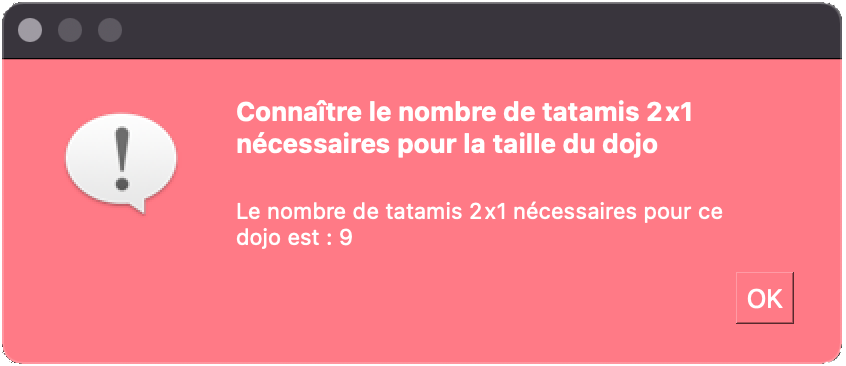
\includegraphics[scale=0.25]{images/prodRetourSucces.png}
          \end{center}


    \item Exemple de message indiquant à l’utilisateur que la demande est impossible avec les dimensions saisies:

          \begin{center}
              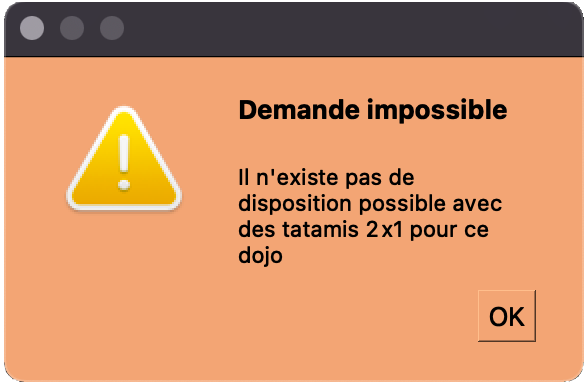
\includegraphics[scale=0.25]{images/prodImpossible.png}
          \end{center}


    \item Exemple de message d’erreur en cas de non saisie ou saisie nulle de dimensions:

          \begin{center}
              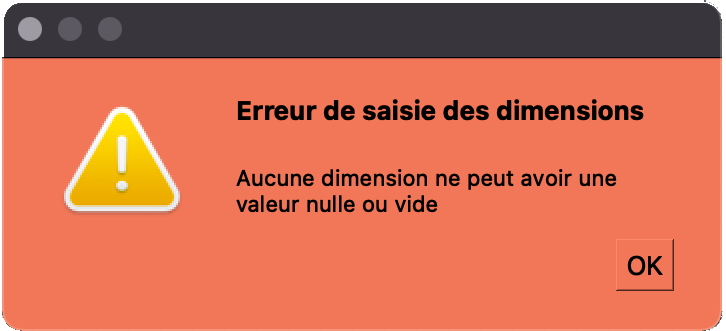
\includegraphics[scale=0.25]{images/prodErreurSaisie.png}
          \end{center}


\end{itemize}
L’interface principale a subi quelques modifications de design (couleur du texte) et l’ajout des boutons pour les
fonctionnalités supplémentaires:

\begin{center}
    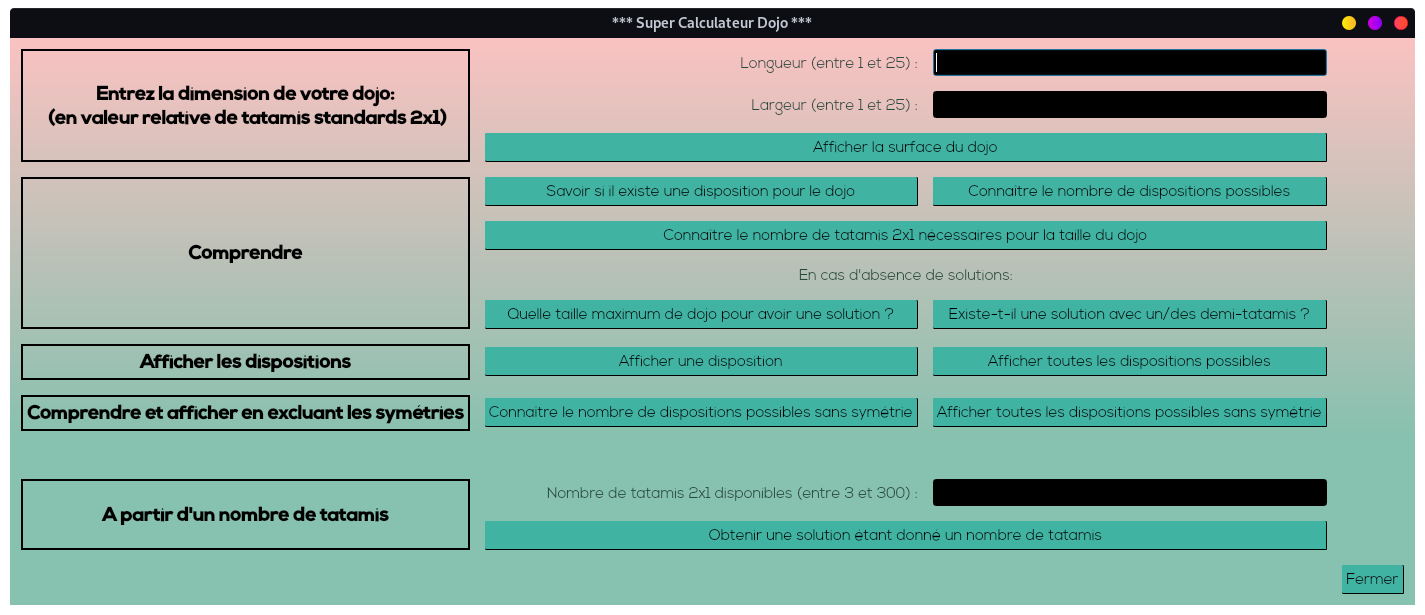
\includegraphics[scale=0.25]{images/prodInterface.png}
\end{center}

\subsection{Choix de la structure du programme}

% Aucun changement majeur n’a été appliqué. Le fichier \texttt{release.py} change de nom et devient
%  \texttt{prod.py} mais son sens reste le même.

Afin de produire un ensemble cohérent et compréhensible de modules pour la livraison du projet, 
un renommage a été effectué :
\begin{itemize}
    \item le module \texttt{calcul\_nombre\_dispositions} a été renommé en \texttt{denombrement} ;
    \item le module \texttt{calcul\_coordonnees\_tatamis} a été renommé en \texttt{pavage} ;
    \item le module \texttt{release} a été renommé en \texttt{main} et prend en charge maintenant le lancement de l'interface;
\end{itemize}

Du refactoring a été implémenté pour améliorer le code, en cohérence avec l’application des principes SOLID:
\begin{itemize}
    \item Un refactoring mineur a été effectué sur le fichier Interface, les messages pop-up d’erreur ont été rationalisés pour passer
          de 5 à 3 et simplement modifier les paramètres de textes changeants quand on les affichent.
    \item Avec l’ajout des fonctions “Connaître le nombre de dispositions possibles sans symétries", la fonction pour exécuter ressemble
          beaucoup aux fonctions “Savoir si il existe un dojo” et “Connaître le nombre de dispositions possibles”. Un refactoring a donc été
          implémenté pour mutualiser une fonction commune pour le click sur ces 3 boutons.
    \item Un refactoring a été implémenté pour corriger la fonction permettant de déterminer les dimensions à partir d'un nombre de tatamis. D'une part
          cette fonction n'était pas correcte puisque ne permettant pas de répondre au critère du taux de 75\% de tatamis utilisés, d'autre part elle était redondante
          et comportait des boucles évitables.

\end{itemize}

\section{Challenges rencontrés et apprentissage}

\subsection{Challenges rencontrés et solutions appliquées}

Ce sprint n’a pas vu apparaître de nouveau challenges. Avec les leçons apprises des précédents sprints, sur l’organisation de l'équipe,
la planification… nous constatons que cela porte ses fruits.

Deux challenges mineurs peuvent être cités:
\begin{itemize}
    \item Technique
          \begin{itemize}
              \item Une nouvelle fois, les ambitions en termes de fonctionnalités restent élevées. En particulier la fonctionnalité
                    d'identification des symétries, comme on peut le constater dans le paragraphe d’explication, l’algorithme doit couvrir
                    de nombreux cas de figure : symétrie d’axe horizontale, d’axe vertical , ainsi que la composition de celles-ci (symétrie centrale).
                    Il a donc fallu s’assurer de pouvoir produire des symétriques de dojo, mais surtout de pouvoir modéliser les dispositions de façon
                    à comparer leur géométrie.
              \item Cela a été en particulier vrai pour la fonctionnalité 526, censée afficher les dojos avec des couleurs différentes pour faciliter
                    la compréhension de l’affichage des dispositions. Compte tenu de la difficulté algorithmique et du manque de temps, il a été décidé
                    d’abandonner cette fonctionnalité.

          \end{itemize}
    \item Rédactionnel

          S’agissant de la fin du projet, et bien qu’ayant écrit le rapport au fur et à mesure des précédents sprint, ce sprint a également été
          l’occasion d’un travail rédactionnel sur le rapport qui est consommateur de temps.

\end{itemize}

\subsection{Apprentissage}

Les principales leçons de ce sprint sont plutôt des confirmations que des apprentissages:
\begin{itemize}
    \item D'itérations et l'amélioration continue portent leurs fruits. Comme mentionné, les leçons apprises lors des précédents sprint
          ont permis d'améliorer l'exécution de notre dernier sprint
    \item La progression au fur et à mesure sur le rapport lors des précédents sprint a également été crucial; il aurait autrement été
          difficile de bien rédiger le rapport dans le temps imparti
\end{itemize}

